% CS6140 Homework Assignment Template
% Computer Science
% Northeastern University
% Boston, MA 02115

% Do not manipulate any of the settings
\documentclass[twoside]{article}

\usepackage{epsfig}
\usepackage{natbib}
\usepackage{units}
\usepackage{amssymb}
\usepackage{amsmath}
\usepackage{babel}
\usepackage{tikz}


\setlength{\oddsidemargin}{0 in}
\setlength{\evensidemargin}{0 in}
\setlength{\topmargin}{-0.6 in}
\setlength{\textwidth}{6.5 in}
\setlength{\textheight}{8.5 in}
\setlength{\headsep}{0.75 in}
\setlength{\parindent}{0 in}
\setlength{\parskip}{0.1 in}

\newcommand{\lecture}[3]{
   \pagestyle{myheadings}
   \thispagestyle{plain}
   \newpage
   \setcounter{page}{1}
   \noindent
   \begin{center}
   \framebox{
      \vbox{\vspace{2mm}
    \hbox to 6.28in { {\bf CS6140: Machine Learning\hfill} }
       \vspace{6mm}
       \hbox to 6.28in { {\Large \hfill #1  \hfill} }
       \vspace{6mm}
       \hbox to 6.28in { {\it Assigned: #2 \hfill Due: #3} }
      \vspace{2mm}}
   }
   \end{center}
   \markboth{#1}{#1}
   \vspace*{4mm}
}

\begin{document}

% to have alphanumeric enumeration (Hasan's command)
\renewcommand{\labelenumi}{\alph{enumi})}

\lecture{Homework Assignment \# 4}{03/26/2021}{04/12/2021, 11:59pm, through Canvas}



%%
%% Problem
%%

\textbf{Problem 1.} (15 points) Consider a logistic regression problem where $\mathcal{X} = \mathbb{R}^d$ and $\mathcal{Y} = \left\{ -1, +1\right\}$. Derive the weight update rule that maximizes the conditional likelihood assuming that a data set $\mathcal{D}=\left\{ (\boldsymbol{x}_{i},y_{i})\right\} _{i=1}^{n}$ is given.

\begin{equation*}
\begin{split}
\theta = (b, w) \\
g(x) = b + \sum_d w_d x_d = b +w^Tx \\
\sigma(a) = \frac{1}{1+e^{-a}} \\
p(y = 1|x;\theta) = \sigma(g(x))\\
LCL = \sum_{i=1}^n \log L(\theta; y_i | x_i) = \sum_{i=1}^n \log f(y_i | x_i; \theta) \\
\textsf{if } y_i = +1 \textsf{ then } LCL = \sigma (g(x)) \textsf{ else } LCL = 1- \sigma(g(x)) \\
p(y_i|x_i; \theta) = \sigma (g(x)^{\frac{y_n+1}{2}}(1 - \sigma (g(x))^{\frac{1-y_n}{2}} \\
log{P(\mathcal{D})} = \sum_n \{ (\frac{y_n+1}{2})\log{\sigma (b +w^Tx)}+(\frac{1-y_n}{2})\log{(1 - \sigma (+w^Tx))}\} \\
\textsf{Lets say b is a part of w such that } w_0 = b \textsf{ and append a 1 to begining of x such that } x_0 = 1 \\
log{P(\mathcal{D})} = \sum_n \{ (\frac{y_n+1}{2})\log{\sigma (w^Tx)}+(\frac{1-y_n}{2})\log{(1 - \sigma (w^Tx))}\} \\
\epsilon(w) =  - \sum_n \{ (\frac{y_n+1}{2})\log{\sigma (w^Tx)}+(\frac{1-y_n}{2})\log{(1 - \sigma (w^Tx))}\} \\
\frac{\partial\epsilon(w)}{\partial w} = \sum_n \{(\frac{y_n+1}{2})(1-\sigma(w^Tx))x_n - (\frac{1-y_n}{2}))(\sigma(w^Tx))(x_n)\} \\
= \sum_n \{\sigma(w^Tx) - y_n\}x_n \\
w^{t +1} = w^{t} - \alpha(\sum_n \{\sigma(w^Tx) - y_n\}x_n ) \\
\textsf{Where } \alpha \textsf{ is the step size and } \alpha > 0
\end{split}
\end{equation*}

%%
%% Problem
%%

\textbf{Problem 2.} (20 points) Consider a logistic regression problem with its initial solution obtained through the OLS regression; i.e., $\mathbf{w}^{(0)}=(\mathbf{X}^{T}\mathbf{X})^{-1}\mathbf{X}^{T}\mathbf{y}$
, in the context of the code provided in class (week 6). Recall that $\mathbf{x}$ was drawn from a mixture of two Gaussian distributions with dim$\left\{ \mathbf{x}\right\}=2$ (before adding a column of ones) and that $y \in \left\{ 0, 1\right\}$. You probably noticed that the initial separation line is consistently closer to the data points of class 0.

\begin{enumerate}
\item (10 points) Why was this the case? Draw a picture (if possible) to support your argument.
\item (5 points) Devise a better initial solution by modifying the standard formula $\mathbf{w}^{(0)}=(\mathbf{X}^{T}\mathbf{X})^{-1}\mathbf{X}^{T}\mathbf{y}$.
\item (5 points) Now again consider the case where $y \in \left\{ -1, +1\right\}$. What is the form of the
modified solution from part (b) in this case?
\end{enumerate}

%%
%% Problem
%%

\textbf{Problem 3.} (40 points) Consider two classification concepts given in Figure 1, where $x\in\mathcal{X}=[-6,6]\times[-4,4]$, $y\in\mathcal{Y}=\left\{-1,+1\right\}$ and $p(y|x) \in \left \{0,1\right \}$ is defined in the drawing. 

\begin{figure}[h]
\centering
\includegraphics[width=\linewidth]{graphic.jpg}
\caption{Two concepts where examples that fall within any of the three $3\times3$ (panel A) or $1\times1$ (panel B) squares are labeled positive and the remaining examples (outside each of the squares but within $\mathcal{X}$) are labeled negative. The position of the point $x=(x_1,x_2)$ in the upper left-hand corner for each square is shown in the picture. Consider horizontal axis to be $x_1$ and vertical axis as $x_2$.}
\label{fig:homology}
\end{figure}

Your experiments in this question will rely on generating a data set of size $n\in\left\{250, 1000, 10000\right\}$ drawn from a uniform distribution in $\mathcal{X}$ and labeled according to the rules from Figure 1; e.g., $P(Y=1|x)=1$ if $x$ that was randomly drawn is inside any of the three squares in either of the two panels, and $P(Y=1|x)=0$ otherwise. The goal of the following two problems will be to train and evaluate classifiers created from the data generated in this way. You can use any library you want in this assignment and do programming in Python, MATLAB, R or C/C++. Your code should be easy to run for each question and sub-question below so that we can replicate your results to the maximum extent possible.

Consider single-output feed-forward neural networks with one or two hidden layers such that the number of hidden neurons in each layer is $h_1\in\left\{1, 4, 12\right\}$ and $h_2\in\left\{0, 3\right\}$, respectively, with $h_2=0$ meaning that there is no second hidden layer. Consider one of the standard objective functions as your optimization criterion and use early stopping and regularization as needed. Consider a hyperbolic tangent activation function in each neuron and the output but you are free to experiment with others if you'd like to. For each of the architectures, defined by a parameter combination $(h_1,h_2)$, evaluate the performance of each model using classification accuracy, balanced accuracy, and area under the ROC curve as your two performance criteria. To evaluate the performance of your models use cross-validation. However, to evaluate the performance of performance evaluation, generate another very large data set on a fine grid in $\mathcal{X}$. Then use the predictions from your trained model on all these points to determine the ``true'' performance. You can threshold your predictions in the middle of your prediction range (i.e., at $0.5$ if you are predicting between 0 and 1) to determine binary predictions of your models and to then compare those with true class labels you generated on the fine grid. 

Provide meaningful comments about all aspects of this exercise (performance results for different network architectures, accuracy of cross-validation, run time, etc.). The comments should not just re-state the results but rather capture trends and give reasoning as to why certain behavior was observed.


For this problem the experiment was set up, with generating the datasets for the sizes $n \in \{ 250, 1000, 10000\} $, then for each of these datasets the process went through the sci-kit learn MLPclassifier or multi-layer perceptron  classifier. The classifier was then tasked to predicted based on k-fold cross validation and the performance results were then obtained through those predictions.  The results were then averaged across all folds. Unsurprisingly the larger datsets and the larger networks took longer to train. Surprisingly the two layer (12, 3) network did not out perform the (12,) in each datset. Seemingly the most confounding variable to which model performed better seemed to be the dataset size rather than the individual layer makeup. The addition of another layer did not seem to showcase that there would be an increase in performance. 

%%
%% Problem
%%

\textbf{Problem 4.} (70 points) Matrix factorization with applications. Consider an $n\times d$ real-valued data matrix $\mathbf{X}=(\mathbf{x}_{1}^{T},\mathbf{x}_{2}^{T},\ldots,\mathbf{x}_{n}^{T})$. We will attempt to approximate this matrix using the following factorization
\[
\hat{\mathbf{X}}=\mathbf{U}\mathbf{V}^{T}
\]
where $\mathbf{U}=(\mathbf{u}_{1}^{T},\mathbf{u}_{2}^{T},\ldots,\mathbf{u}_{n}^{T})$ is an $n\times k$ and $\mathbf{V}=(\mathbf{v}_{1}^{T},\mathbf{v}_{2}^{T},\ldots,\mathbf{v}_{d}^{T})$ is a $d\times k$ matrix of real numbers, and where $k<n,d$ is a parameter to be explored and determined. Notice that the value $x_{ij}$ in \textbf{$\mathbf{X}$} can be approximated by $\mathbf{u}_{i}^{T}\mathbf{v}_{j}$ and that $\mathbf{x}_{i}^{T}$, the $i$-th row of $\mathbf{X}$, can be approximated by $\mathbf{u}_{i}^{T}\mathbf{V}^T$, giving $\hat{\mathbf{x}}_{i}=\mathbf{V}\mathbf{u}_{i}$. We will formulate the matrix factorization process as the following minimization
\[
\underset{\mathbf{U},\mathbf{V}}{\min}\sum_{i,j}(x_{ij}-\mathbf{u}_{i}^{T}\mathbf{v}_{j})^{2}+\lambda(\sum_{i}||\mathbf{u}_{i}||^{2}+\sum_{j}||\mathbf{v}_{j}||^{2})
\]
which minimizes the sum-of-squared-errors between real values $x_{ij}$ and reconstructed values  $\hat{x}_{ij}=\mathbf{u}_{i}^{T}\mathbf{v}_{j}$. The regularization parameter $\lambda\geq0$ is user-selected. This problem can be directly solved using gradient descent, but we will attempt a slightly different approach. To do this, we can see that for a fixed $\mathbf{V}$ we can find optimal vectors $\mathbf{u}_{i}$ by minimizing
\[
||\mathbf{V}\mathbf{u}_{i}-\mathbf{x}_{i}||^{2}+\lambda\cdot||\mathbf{u}_{i}||^{2}
\]
which can be solved in a closed form using OLS regression for every $i$. We can equivalently express the optimization for vectors $\mathbf{v}_{j}$ and find the solution for every $j$. Then, we can alternate these steps until convergence. This procedure is called the Alternating Least Squares (ALS) algorithm for matrix factorization. It has the following steps:

$\quad\quad$Initialize $\mathbf{U}$  and $\mathbf{V}$

\vspace{-0.75em}

$\quad\quad$\textbf{repeat}

\vspace{-0.75em}

$\quad\quad\quad\quad$\textbf{for} $i=1$ to $n$

\vspace{-0.75em}

$\quad\quad\quad\quad\quad\quad\mathbf{u}_{i}=\textrm{ formula \#1}$

\vspace{-0.75em}

$\quad\quad\quad\quad$\textbf{end}

\vspace{-0.75em}

$\quad\quad\quad\quad$\textbf{for} $j=1$ to $d$

\vspace{-0.75em}

$\quad\quad\quad\quad\quad\quad\mathbf{v}_{j}= \textrm{ formula \#2}$

\vspace{-0.75em}

$\quad\quad\quad\quad$\textbf{end}

\vspace{-0.75em}

$\quad\quad$\textbf{until} convergence

\noindent where you are expected to derive formula \#1 and formula \#2.

\begin{enumerate}
\item (10 points) Derive the optimization steps for the ALS algorithm by finding formula \#1 and formula \#2 in the  pseudocode listed above. 

formula \#1 = 
\begin{equation*}
\begin{split}
\frac{\partial}{\partial u_i}\underset{\mathbf{U},\mathbf{V}}{\min}\sum_{i,j}(x_{ij}-\mathbf{u}_{i}^{T}\mathbf{v}_{j})^{2}+\lambda(\sum_{i}||\mathbf{u}_{i}||^{2}+\sum_{j}||\mathbf{v}_{j}||^{2}) & = \\
& = -2\sum_j\left(x_{ij} - u^T_i v_j\right)v^T_j +  \lambda_u u_i^T \\
0 & = -\left(x_{i} - u^T_iV^T\right)V + 2 \lambda_u u_i^T \\
u_i^T(V^T V + \lambda_u \mathbb{I}) & = x_iV \\
u_i^T  & = x_iV(V^TV + \lambda_u \mathbb{I})^{-1} \\
u_i &= (V^TV + \lambda_u \mathbb{I})^{-1} \times V^Tx_i
\end{split} 
\end{equation*}


formula  \#2 =
\begin{equation*}
\begin{split}
\frac{\partial}{\partial v_j}\underset{\mathbf{U},\mathbf{V}}{\min}\sum_{i,j}(x_{ij}-\mathbf{u}_{i}^{T}\mathbf{v}_{j})^{2}+\lambda(\sum_{i}||\mathbf{u}_{i}||^{2}+\sum_{j}||\mathbf{v}_{j}||^{2}) & = \\
& = -2\sum_i\left(x_{ij} - v^T_j u_i\right)u^T_i + \lambda_v v_j^T \\
0 & = -\left(x_{i} - v^T_jU^T\right)U + 2 \lambda_vv_j^T \\
v_j^T(U^T U + \lambda_v \mathbb{I}) & = x_iU \\
v_j^T  & = x_iU(U^TU + \lambda_v \mathbb{I})^{-1} \\
v_j & = (U^TU+ \lambda_v \mathbb{I})^{-1} \times U^Tx_i
\end{split} 
\end{equation*}
\item (20 points) Consider now that some values in $\mathbf{X}$ are missing (e.g., the rows of $\mathbf{X}$ are users and the columns of $\mathbf{X}$ are movie ratings, when available) and that we are interested in carrying out matrix completion using matrix factorization presented above. We would like to use the ALS algorithm, but the problem is that we must exclude all missing values from optimization. Derive now a modified ALS algorithm (formulas \#1 and \#2) to adapt it for matrix completion. Hint: consider adding an indicator matrix $\mathbf{W}$ to the optimization process, where $w_{ij}=1$ if $x_{ij}$ is available and $w_{ij}=0$ otherwise.

\begin{equation*}
\begin{split}
\frac{\partial}{\partial}\underset{\mathbf{U},\mathbf{V}}{\min}\sum_{i,j}w_{i,j}(x_{ij}-\mathbf{u}_{i}^{T}\mathbf{v}_{j})^{2}+\lambda(\sum_{i}||\mathbf{u}_{i}||^{2}+\sum_{j}||\mathbf{v}_{j}||^{2}) & = \\
\end{split} 
\end{equation*}
w.r.t. $v_j$ and $u_i$ just as above

\begin{equation*}
\begin{split}
u_i &=  (V^Tw_iV + \lambda_u \mathbb{I})^{-1} \times V^Tw_ix_i\\
v_j & = (U^Tw_jU+ \lambda_v \mathbb{I})^{-1} \times U^Tw_jx_i
\end{split} 
\end{equation*}

\item (20 points) Consider now a MovieLens database available at

\begin{center}
\texttt{http://grouplens.org/datasets/movielens/}
\end{center}

and find a data set most appropriate to evaluate your algorithm from the previous step; e.g., one of the 100k data sets. Now, implement the ALS algorithm on your data set and evaluate it using the mean-squared-error as the criterion of success. You can randomly remove 25\% of the ratings, train a recommendation system, and then test it on the test set. You will have to make certain decisions yourselves, such as initialization of $\mathbf{U}$ and $\mathbf{V}$, convergence criterion, or picking $k$ and $\lambda$.

\item (10 points) Describe your full experimentation process (e.g., how did you vary $k$) and observations from (c). Additionally, can you provide some reasoning as to what $k$ is and what matrices $\mathbf{U}$ and $\mathbf{V}$ are?

For this process I loaded the data file from the movielens dataset, removed 25\% of the reviews and then pivoted the data so that the data was in a $i$ by $j$ matrix. I filled all null values with 0. I then used sci-kit learns non-negative matrix factorization to return the 2 compositional matrices which were size of $i$ by $k$ and $k$ by $j$ respectively. The final predicted matrix could then be found by finding the dot product of these 2 matrices.
For this experiment i tried 5 different values of k; $k \in [10, 20, 40, 80, 100] $. From my experimentation k represents latent or derived variables and the U and V matrix are the the latent variables the users and the movies respectively. The MSE decreased after the initial increase of k from 10 to 20 but increased with every increase there after showcasing to me that there is some sweet spot for which k minimizes the MSE. 
\begin{table}[]
\begin{tabular}{ll}
K   & MSE   \\
10  & 7.254 \\
20  & 7.204 \\
40  & 7.730 \\
80  & 8.849 \\
100 & 9.254
\end{tabular}
\end{table}

\item (10 points) Compare your method against the baseline that fills in every missing movie rating value $x_{ij}$ as an average over all users who have rated the movie $j$. Discuss your empirical findings.

For the average after the 25\% were removed some movies ended up with no ratings for those movies those ratings were filled in with 0 for this baseline. The MSE for this baseline was 1.067 which is significantly lower than any of the values for the models made with matrix factorization. I find this very interesting and wonder if it has to do with the number of empty values within the matrix since the movielens dataset only contained 100,000 entries but the matrix was a size of 1.5 million rating entries. 

\end{enumerate}

%%
%% Problem
%%

\textbf{Problem 5.} (15 points) Prove representational equivalence of a three-layer neural network with linear activation function in all neurons and a single-layer layer neural network with the same activation function. Assume a single-output network.

%%
%% Problem
%%

\textbf{Problem 6.} (10 points) Let $A$, $B$, $C$, and $D$ be binary input variables (features). Give decision trees to represent the following Boolean functions:

\begin{enumerate}
\item (3 points) $A\wedge \bar{B}$
\item (3 points) $A\vee(\bar{B}\wedge C)$
\item (4 points) $A \oplus \bar{B}$
\end{enumerate}
where $\bar{A}$ is the negation of $A$ and $\oplus$ is an exclusive OR operation.

\tikzset{
treenode/.style = {align=center},
c/.style = {treenode,circle,draw=black,minimum width=1.5em,minimum height=1.5em,text centered,font=\footnotesize},
r/.style = {treenode,rectangle,draw=black,minimum width=1.5em,minimum height=1.5em,text centered,font=\footnotesize},
level 1/.style={sibling distance=60mm},
level 2/.style={sibling distance=30mm},
level 3/.style={sibling distance=15mm},
level 4/.style={sibling distance=7mm}
}

a)

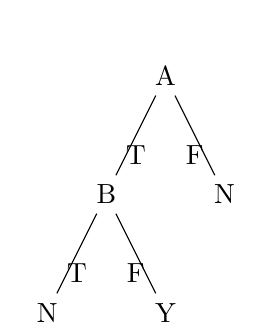
\begin{tikzpicture}
    \node {A}
	child { node {B}
		child {node {N}
		  edge from parent node [below]{T} }
		child {node {Y}
		  edge from parent node [below]{F} }
      edge from parent node [below] {T} 
      }
    child { node {N}
      edge from parent node[below] {F} }
    ;
\end{tikzpicture}

b)


\begin{tikzpicture}
    \node {A}
    child { node {Y}
      edge from parent node [below]{T} }
	child { node {B}
		child {node {N}
		  edge from parent node[below]{T} }
		child {node {C}
		   child {node {Y}
			   edge from parent node [below]{T} }
	       child { node {N}
	           edge from parent node [below]{F} }
	       edge from parent node [below]{F}}		
      edge from parent node [below]{F} 
      }
    ;
\end{tikzpicture}

c)

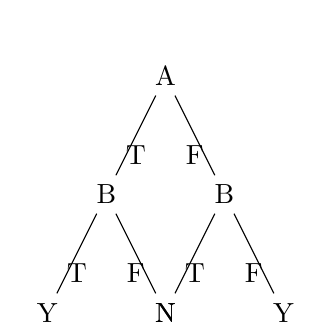
\begin{tikzpicture}
    \node {A}
	child { node {B}
		child {node {Y}
		  edge from parent node[below]{T} }
		child {node {N}
		  edge from parent node[below]{F} }
      edge from parent node [below]{T} 
      }
 	child { node {B}
		child {node {N}
		  edge from parent node[below]{T} }
		child {node {Y}
		  edge from parent node[below]{F} }
      edge from parent node [below]{F} 
      }
    ;
\end{tikzpicture}

\end{document}
